\section{Experimentos}\label{section_experimento}

Como forma de avaliar o modelo proposto serão conduzidos dois principais experimentos.

\subsection{Experimento 1: Formação de assembleias neuronais}

O primeiro experimento consiste em simular a RNP apresentando estímulos ao modelo de retina e analisar se a repetição dos
estímulos leva à formação de assembleias neuronais associadas a cada estímulo a longo prazo, com o objetivo de ter uma base de
comparação para o experimento 2, que terá o sono simulado. Os estímulos consistem em seis imagens simples de serem reconhecidas,
exibidas na Figura~\ref{fig_estimulos}, e são apresentados à rede de forma intercalada e aleatória. Quatro estímulos foram
reaproveitados do trabalho de~\citeonline{zenkeDiverse2015}, enquanto as figuras de diamante e de cruz foram adicionadas com o
intuito de colocar a RNP mais próxima do seu limite.

\begin{figure}[!ht]
\caption{Os seis estímulos apresentados à RNP durante os experimentos.}
\centering{
\parbox{12cm}{
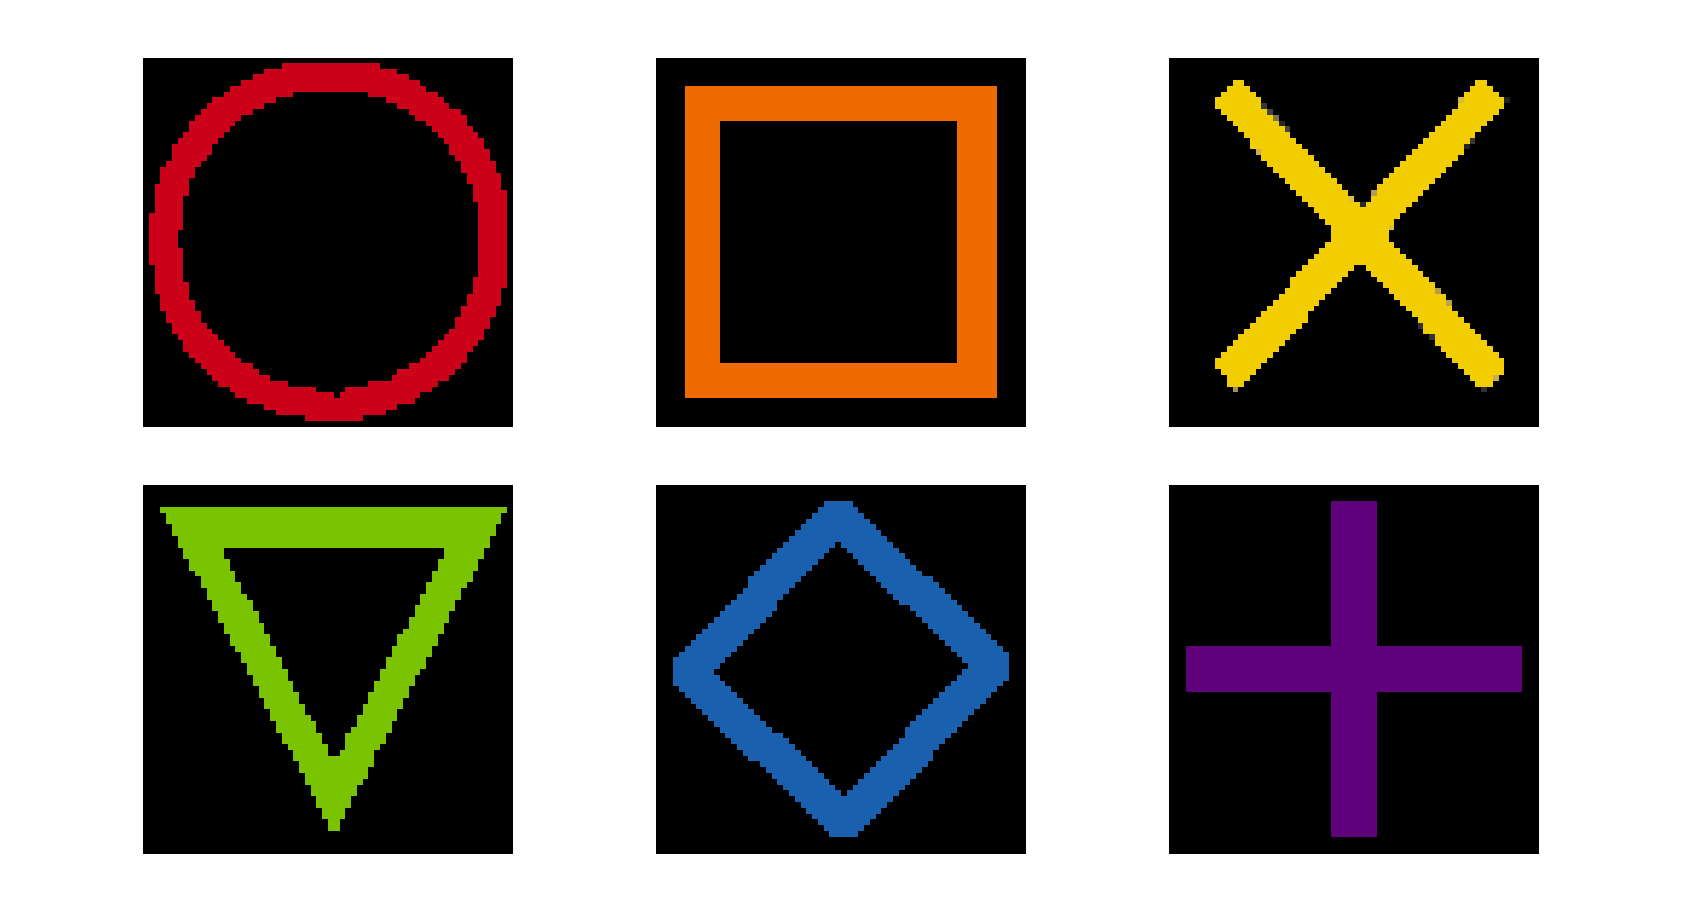
\includegraphics[width=12cm]{figuras/estimulos_cor.png}\label{fig_estimulos}
\fonte{Elaborado pelo autor (2023).}}}
\end{figure}

Houveram três fases da simulação da RNP:

\begin{enumerate}
  \item Simulação da rede em seu estado inicial por 1800 segundos, com um tempo médio de aparição do estímulo de 2 segundos, e
  tempo médio entre estímulos de 1 segundo. O peso das sinapses entre a retina e a rede é de 0.05.
  \item Simulação da rede também por 1800 segundos, mas com um tempo médio de aparição do estímulo de 0.2 segundo, e
  tempo médio entre estímulos de 5 segundos. O peso das sinapses entre a retina e a rede agora é de 0.1. A intenção aqui é
  fazer com que a rede tenha mais tempo entre um estímulo e outro para poder memorizá-los melhor.
  \item A última simulação é de 2400 segundos e é de onde são tirados os resultados. O tempo médio de aparição do estímulo diminui
  para 0.1, enquanto o tempo médio entre estímulos é de 10 segundos, com a intenção de ter uma janela maior de tempo entre os
  estímulos para analisar a capacidade de memorização da RNP.
\end{enumerate}


\subsection{Experimento 2: Formação de assembleias neuronais com sono}

De forma similar ao experimento 1, o segundo experimento consiste em simular a RNP apresentando os mesmos estímulos, mas dessa vez
com a simulação de sono. O objetivo desse experimento é analisar se a simulação de sono tem algum efeito na formação de
assembleias neuronais.

Esse experimento seguiu as mesmas três fases do experimento anterior, mas com a simulação do sono. Nesse experimento, a RNP ficava
em estado de vigília por 400s e dormia por 200s.

\section{Análise}

A parte final do trabalho consistirá em analisar as diferentes simulações feitas e determinar se a simulação de sono teve algum
efeito na formação de assembleias neuronais. Para isso, antes de tudo é necessário um modo de identificar as assembleias neuronais
e quais neurônios pertencem a cada uma.

Para determinar quais neurônios pertencem à assembleia neuronal associada a um estímulo, será analisada a frequência de disparos de
cada neurônio no intervalo $3s < t < 3.5s$ após a apresentação do estímulo. Os neurônios que disparam com frequência maior que
10Hz serão considerados como pertencentes à assembleia neuronal associada a um estímulo.

Por fim, será analisado quanto tempo leva para a assembleia neuronal associada ser formada e quanto tempo ela dura nas diferentes
simulações.


